\documentclass{standalone}
\usepackage{tikz}
\usetikzlibrary{arrows.meta,decorations.markings}

\begin{document}
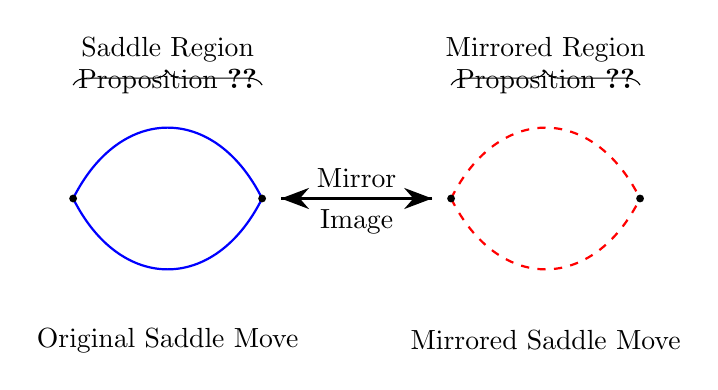
\begin{tikzpicture}[scale=1.2,
    saddle/.style={thick, blue},
    mirror/.style={thick, red, dashed},
    handle/.style={circle, fill, inner sep=1pt},
    >={Stealth[scale=1.2]}
]

% Original saddle move
\draw[saddle] (0,0) .. controls (0.5,1) and (1.5,1) .. (2,0);
\draw[saddle] (0,0) .. controls (0.5,-1) and (1.5,-1) .. (2,0);
\node[handle] at (0,0) {};
\node[handle] at (2,0) {};

% Mirror image
\begin{scope}[xshift=4cm, yscale=-1]
    \draw[mirror] (0,0) .. controls (0.5,1) and (1.5,1) .. (2,0);
    \draw[mirror] (0,0) .. controls (0.5,-1) and (1.5,-1) .. (2,0);
    \node[handle] at (0,0) {};
    \node[handle] at (2,0) {};
\end{scope}

% Arrows connecting corresponding elements
\draw[->, very thick] (2.2,0) -- (3.8,0) node[midway, above] {Mirror};
\draw[->, very thick] (3.8,0) -- (2.2,0) node[midway, below] {Image};

% Labels
\node[above] at (1,1) {Proposition \ref{prop:newii}};
\node[above] at (5,1) {Proposition \ref{prop:newimirror}};
\node at (1,-1.5) {Original Saddle Move};
\node at (5,-1.5) {Mirrored Saddle Move};

% Decoration
\draw[decorate,decoration={brace,amplitude=5pt}] (0,1.2) -- (2,1.2) 
    node[midway,above=5pt] {Saddle Region};
\draw[decorate,decoration={brace,amplitude=5pt}] (4,1.2) -- (6,1.2)
    node[midway,above=5pt] {Mirrored Region};

\end{tikzpicture}

% Explanatory text
\begin{tikzpicture}[overlay, remember picture]
\node[align=left, text width=10cm] at (5,-3) {
    The saddle moves of Proposition \ref{prop:newii} are consistent under mirror image. 
    The diagram shows the original saddle configuration (left) and its mirror image (right). 
    The mirror operation preserves the essential topological structure while reversing orientation, 
    as demonstrated in the proof of Proposition \ref{prop:newimirror}.
};
\end{tikzpicture}
\end{document}